% !TeX root = Documentation.tex
\documentclass[german,report,noglossaries]{hbrs-thesis}

\begin{document}
\begin{titlepage}
    \begin{center}
        {\LARGE Dokumentation zu \texttt{hbrs-thesis}}
        \vfill
        {\Huge \textit{Modern und wissenschaftlich}}
        \vfill
        {\LARGE Version 1.0}\\
        \vspace{2em}
        {\Large \today}
    \end{center}
\end{titlepage}

\tableofcontents
% \listofcode

\chapter{Vorwort}
Diese Dokumentation ist nicht vollumfänglich. Das bedeutet, dass sie nicht auf alle Eigenheiten der einzelnen verwendeten Pakete eingeht. Für weitere und aktuelle Informationen empfehle ich immer die Recherche auf \url{https://www.ctan.org/}, wo alle Pakete mit ihren Dokumentationen hinterlegt sind.

In diesem Dokument werden die wichtigsten Befehle gezeigt und erklärt. Diese Dokumentation kann und sollte gerne durch die Hilfe der Community korrigiert und erweitert werden.

Viel Erfolg beim Schreiben!
\chapter{Verwendung der \LaTeX-Klasse}
Um die Klasse als Vorlage für Dokumente zu verwenden, empfiehlt es sich, den kompletten Ordner \texttt{template} zu kopieren und entsprechend dieser Dokumentation zu verwenden. In diesem Kapitel werden die einzelnen Bestandteile des Ordners kurz erklärt. Die Verwendung der einzelnen Ordner und Dateien wird im späteren Verlauf des Dokuments näher erläutert.

\section{Bestandteile des Templates}
Die Konfiguration aller Informationen auf dem Deckblatt, sowie die Widmung können \marginpar{\texttt{assets/\\utility/*}}über die Datei \texttt{assets/utility/meta.tex} angepasst werden. Innerhalb des Ordners \texttt{assets/utility} finden sich außerdem noch eine Datei für Worttrennungen, die von \LaTeX nicht korrekt erkannt werden (\texttt{hyphenation.tex}), Akronyme (\texttt{acronyms.tex}) und Glossareinträge (\texttt{glossary.tex}).

In \texttt{assets/images} werden Bilder hinterlegt. Je nach Anzahl der Bilder im Dokument \marginpar{\texttt{assets/\\images/*}}empfiehlt es sich, diese nach Kapitel zu sortieren. Im Ordner \texttt{assets/images} befindet sich bereits ein Ordner \texttt{titlepage}, welcher die Bilder für die Titelseite enthält. Diese sollten nicht gelöscht werden, da sonst die Titelseite und somit das Dokument nicht mehr gebaut werden kann.

Der Ordner \texttt{chapter} ist dafür gedacht, die Kapitel oder Abschnitte (je nach Verwendung der Dokumentklasse (siehe \autoref{chap:klassenoptionen})) \marginpar{\texttt{chapter}}aufzuteilen und die entsprechenden Dateien dort abzulegen. Diese Aufteilung bringt den Vorteil, dass Kapitel sehr schnell neu sortiert werden können. Zusätzlich enthalten die Dateien weniger Text und sind damit übersichtlicher.

Zu einem wissenschaftlichen Dokument gehört auch Literatur. Die Informationen zu dieser \marginpar{\texttt{biblio-\\graphy.bib}}Literatur werden als BibTeX oder BibLaTeX in der Datei \texttt{bibliography.bib} hinterlegt. Ich persönlich bevorzuge es die PDF-Dokumente lokal mit abzuspeichern. Mit lokalen Dateien habe ich die Möglichkeit Anmerkungen zu machen und die Dateien mit anderer Software besser zu durchsuchen (siehe \url{https://github.com/freedmand/semantra}). Die PDF-Dokumente kommen dann in den dieser \marginpar{\texttt{literature}}Ordner \texttt{literature}. Je nach Literaturverwaltungssoftware können Einstellungen getroffen werden, um diese Dokumente direkt in der Software aufzurufen.

Für den Bau des Dokuments mit \texttt{latexmk} wird die Datei \texttt{.latexmkrc} benötigt, da sie \marginpar{\texttt{.latexmkrc}}Informationen zum Bauen des Dokumentes mit Glossar und Akronymen enthält. Wird kein Glossar- und/oder Akronymverzeichnis benötigt, empfiehlt es sich, die entsprechende Option in der Klasse zu verwenden (siehe \autoref{chap:klassenoptionen}).

Beim Kompilieren des Dokumentes entsteht ein neuer Ordner \texttt{out}. \marginpar{\texttt{out}}Dieser Ordner enthält verschiedene Kompilierungsschritte, Log- und Synchronisierungsdateien von \LaTeX. Im Zweifel kann dieser Ordner gelöscht und der Buildprozess neu gestartet werden. Die darin befindliche PDF-Datei (das gebaute Dokument) sollte jedoch vorher gespeichert werden, um einen Verlust der Daten zu vermeiden. Vorschläge für eine Konfiguration von \LaTeX-Umgebungen in verschiedenen IDEs werden auch noch vervollständigt.

Zuletzt befindet sich in \texttt{hbrs-thesis.cls} sämtliche Konfiguration für die Klassendatei. \marginpar{\texttt{hbrs-\\thesis.cls}}Diese Konfiguration kann nach Belieben angepasst werden. Sollten Grundsätzliche Änderungs- oder Verbesserungsvorschläge an dieser Datei entstehen, bitte ich darum, diese auch bei GitHub (siehe \url{https://github.com/blackapple113/H-BRS-Thesisvorlage}) einzureichen.
\chapter{Optionen der Klasse hbrs-thesis}
\label{chap:klassenoptionen}
Für die Modularität der Klasse wurden einige Optionen eingebaut. Mithilfe dieser Optionen lässt sich das Dokument zum Teil in Optik und Verwendungszweck anpassen. Im Folgenden werden die Optionen mit Beispielen erläutert.

\section{Spracheinstellungen}
Eine Pflichtoption, welche für eine korrekte Worttrennung verwendet werden muss ist die Einstellung der Sprache. Die Sprache kann aktuell nur zwischen englisch und deutsch unterschieden werden. Weitere Anpassungsmöglichkeiten für komplexere bilinguale Dokumente oder andere Spracheinstellungen müssen über die Datei \texttt{hbrs-thesis.cls} manuell eingestellt werden. Angenommen es wird ein Dokument auf Deutsch geschrieben, so muss in Kombination mit dieser Klasse die Option auf \texttt{german} gesetzt werden. Intern werden dann Optionen für die Deutsche Sprache gesetzt. Wird das Dokument auf Englisch geschrieben, so muss \texttt{english} angegeben werden. 

\begin{code}{latex}
\documentclass[german]{hbrs-thesis}
…
\end{code}

Werden bilinguale Spracheinstellungen im Dokument benötigt, müssen in der Klassendatei \texttt{hbrs-thesis.cls} Einstellungen für das Paket \texttt{babel} getroffen werden. Das Paket befindet sich unter der Region \texttt{Required packages}. Ist die Hauptsprache des Dokuments Englisch, kommen aber durchaus Deutsche Begriffe darin vor, eignet sich die Konfiguration \mintinline{latex}{\RequirePackage[ngerman,english]{babel}}. Die zuletzt angegebene Sprache ist die Hauptsprache.

\begin{information}
    Wird die Sprache über die Optionsmöglichkeiten für das Paket \texttt{babel} direkt in \texttt{hbrs-template.cls} geändert, dürfen keine Sprachangaben als Klassenoptionen gesetzt werden.
\end{information}

\section{Stiloptionen}
Die Klasse besitzt ein paar Optionen, um verschiedene Stile anzubieten. Mithilfe der Option \texttt{classicstyle} bzw. \texttt{modernstyle} kann zwischen einer Schriftart mit Serifen und einer serifenlosen Schriftart (was sind Serifen: \url{https://de.wikipedia.org/wiki/Serife}) unterschieden werden. Serifen sollen dem Lesenden helfen die Zeilen besser zu verfolgen, um während des Lesens nicht in der Zeile zu verrutschen, sind aber auf Bildschirmen teilweise schlechter darzustellen. Der Standard ist hier \texttt{modernstyle} und muss somit nicht explizit angegeben.
\begin{showcase}
\begin{code}{latex}
\documentclass[german,classicstyle]{hbrs-thesis}
…
\end{code}
\tcblower
\begin{figure}[H]
    \centering
    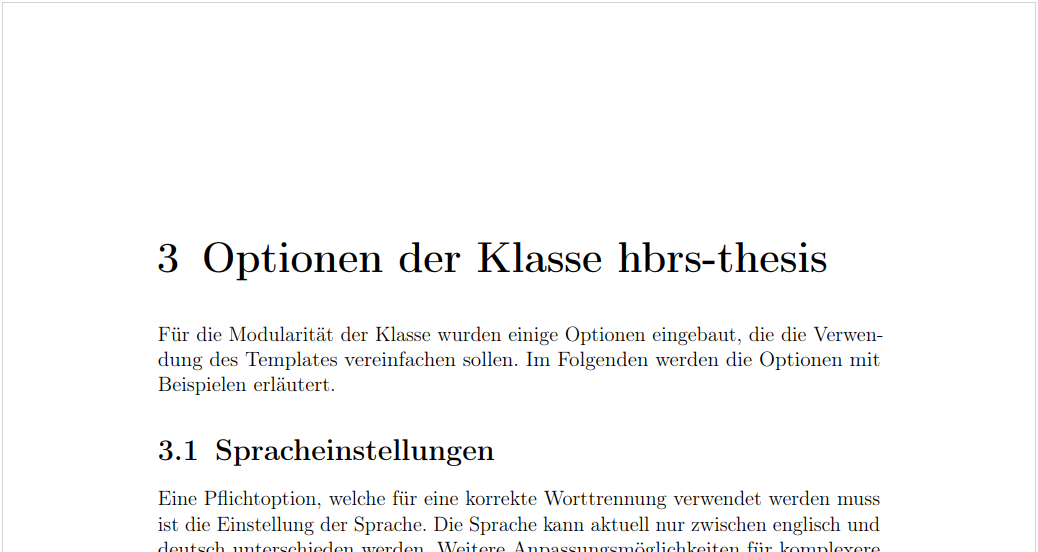
\includegraphics[width=0.8\columnwidth]{assets/images/klassenoptionen/classicstyle.png}
    \caption{Beispielbild für die Option \texttt{classicstyle}.}
\end{figure}
\end{showcase}

Neben dem Stil der Schriftart kann auch zwischen \texttt{report} und \texttt{article} unterschieden werden. Report bietet einzelne Kapitel beschrieben durch \mintinline{latex}{\chapter{…}} welche immer auf einer neuen Seite anfangen. Im Gegensatz dazu bietet \texttt{article} lediglich Abschnitte beschrieben durch \mintinline{latex}{\section{…}}, die nicht jedes Mal auf einer neuen Seite beginnen. Diese beiden Stile können durch die Größe des entstehenden Dokumentes unterschieden werden. Zum Beispiel wird so bei einem Praxisprojektbericht \texttt{article} verwendet wohingegen für eine Thesis \texttt{report} geeignet erscheint. Da die Dokumente nicht doppelseitig ausgedruckt werden entfällt die Option für ein Buchlayout. Diese wird vielleicht später noch hinzugefügt. \textbf{Die Option \texttt{article} ist standardmäßig konfiguriert.} Für eine Thesis sollten die Optionen für die Klasse \texttt{hbrs-thesis} also z.\,B. wie folgt verwendet werden:

\begin{code}{latex}
\documentclass[german,classicstyle,report]{hbrs-thesis}
…
\end{code}

\section{Druckoptionen}
Soll das Dokument ausgedruckt und gebunden werden ergibt sich die Notwendigkeit für einen erweiterten Seitenrand an der Bindeposition (innerer Seitenrand). Mit der Option \texttt{noprint} kann im Dokument explizit angegeben, dass dieses Dokument nicht gedruckt und gebunden wird. So verschiebt sich der Textbereich mittig auf die Seite mit gleichmäßigen Seitenrändern. Standardmäßig ist die \texttt{noprint} Option deaktiviert, da es sich bei der Vorlage um eine Thesisvorlage handelt und diese in der Regel ausgedruckt wird.

\begin{code}{latex}
\documentclass[german,noprint]{hbrs-thesis}
…
\end{code}

\section{Glossar und Akronymverzeichnis}
Werden kein Glossar und/oder Akronymverzeichnis verwendet empfiehlt es sich die Option \texttt{noglossaries} in der Klasse zu verwenden. Damit wird das entsprechende Paket nicht geladen, es wird keine Warnung diesbezüglich ausgegeben und das Kompilieren geht eventuell schneller.

\begin{code}{latex}
\documentclass[german,noglossaries]{hbrs-thesis}
…
\end{code}

\section{Aus PDF kopieren}
Für die bessere Unterstützung des heraus Kopierens von Text aus der fertigen PDF-Datei wird das Paket \texttt{mmap} verwendet. Aufgrund der Einstellungen der Schriftart werden jedoch sehr viele Warnungen ausgegeben, weshalb die Option standardmäßig deaktiviert ist. Um den Lesenden ein einfacheres Kopieren von Inhalten zu ermöglichen, kann das Paket \texttt{mmap} mit der gleichnamigen Option aktiviert werden.

\begin{code}{latex}
\documentclass[german,mmap]{hbrs-thesis}
…
\end{code}
\chapter{Funktionen der Klasse}
In diesem Kapitel werden die wichtigsten integrierten Funktionen der Klasse erklärt und mit Beispielen veranschaulicht. Nochmal der Hinweis, dass nicht sämtliche Funktionen der integrierten Pakete erläuter werden, sondern eine Verwendung innerhalb dieser Klasse für den einfachen Gebrauch dargestellt wird. Optionen der einzelnen Pakete können in \texttt{hbrs-thesis.cls} geändert werden. Dokumentation zu den einzelnen Paketen findet sich auf \url{https://www.ctan.org/}.

\section{Code}
Diese Klasse verwendet das Paket \texttt{minted} (siehe \url{https://www.ctan.org/pkg/minted}) für Syntax Highlighting. Das Paket basiert auf \textit{Pygments} (siehe \url{https://pygments.org/}) welches mit Python auf dem System installiert sein sollte, solange kein Docker-Container zum Bauen bereitsteht. Außerdem muss für das Kompilieren die Option \texttt{-shell-escape} hinzugefügt werden, also \mintinline{bash}{latexmk -shell-escape file.tex}.

\subsection{Inline Code}
Code, der im Text stehen soll, kann auf verschiedene Arten erreicht werden. Die einfachste ist die Verwendung von \texttt{\textbackslash{}texttt\{…\}}. Dabei wird allerdings kein Syntax Highlighting verwendet. Der Text wird innerhalb dieser Umgebung nur an Leerzeichen umgebrochen und nicht innerhalb der Wörter.

Eine weitere Möglichkeit für Syntax Highlighting im Fließtext bietet \texttt{minted} mit dem Befehl \mintinline{latex}{\mintinline{sprache}{code}}. Dieser Befehl kann zusätzlich an vorgegebenen Stellen den Text umbrechen, was dennoch zu Problemen bei der Formatierung am Rand führen kann.

\subsection{Block Code}
Oft ist es notwendig Programmcode im Dokument darstellen zu können. Für diesen Zweck gibt es zwei verschiedene Möglichkeiten. Zum einen kann der Code direkt in die \LaTeX-Datei geschrieben werden, was bei Änderungen zu manuellen Anpassungen führt. Zum anderen kann der Code auch aus den Dateien importiert werden. \textbf{Aufgrund von Limitierungen von minted und TeX kann es zur Ausführung von Code kommen, weshalb nur bekannter Code geladen werden sollte!}

Code kann wie in \autoref{chap:klassenoptionen} ohne starkes visuelles Absetzen direkt unter den Text geschrieben werden, in dem die Umgebung \texttt{code} verwendet wird.

\begin{code}[latex]
    \begin{code}[python]
        if __name__ == "__main__":
            print("Hello World!")
    \end{…} % ersetze … durch "code"
\end{code}

Um den Code optisch durch Linien klar abzugrenzen, wird die Umgebung \texttt{codeblock} verwendet. Dieser Codeblock eignet sich vor allem für größere Codebereiche.

\begin{code}[latex]
    \begin{codeblock}[python]
        class Test:
            __init__(self):
                self.x = 5

        if __name__ == "__main__":
            print("Hello World!")
    \end{codeblock}
\end{code}

Wie oben schon beschrieben kann Code auch aus anderen Dateien geladen werden. Dies geschieht mithilfe des Befehls \mintinline{latex}{\inputcode{language}{path/to/file}{title}}.

\begin{code}[latex]
    \inputcode{java}{assets/code/Test.java}{inputcode}
\end{code}


\end{document}